% ============================================================
%  Slide 2: t-SNE view of learned jet embeddings
% ============================================================
\begin{frame}[plain]
  \slideheader{Visualizing jet embeddings}
  \setbeamerfont{itemize/enumerate body}{size=\footnotesize}

  \vfill
  \begin{columns}[c,onlytextwidth]
    \begin{column}{0.66\textwidth}
      \centering
      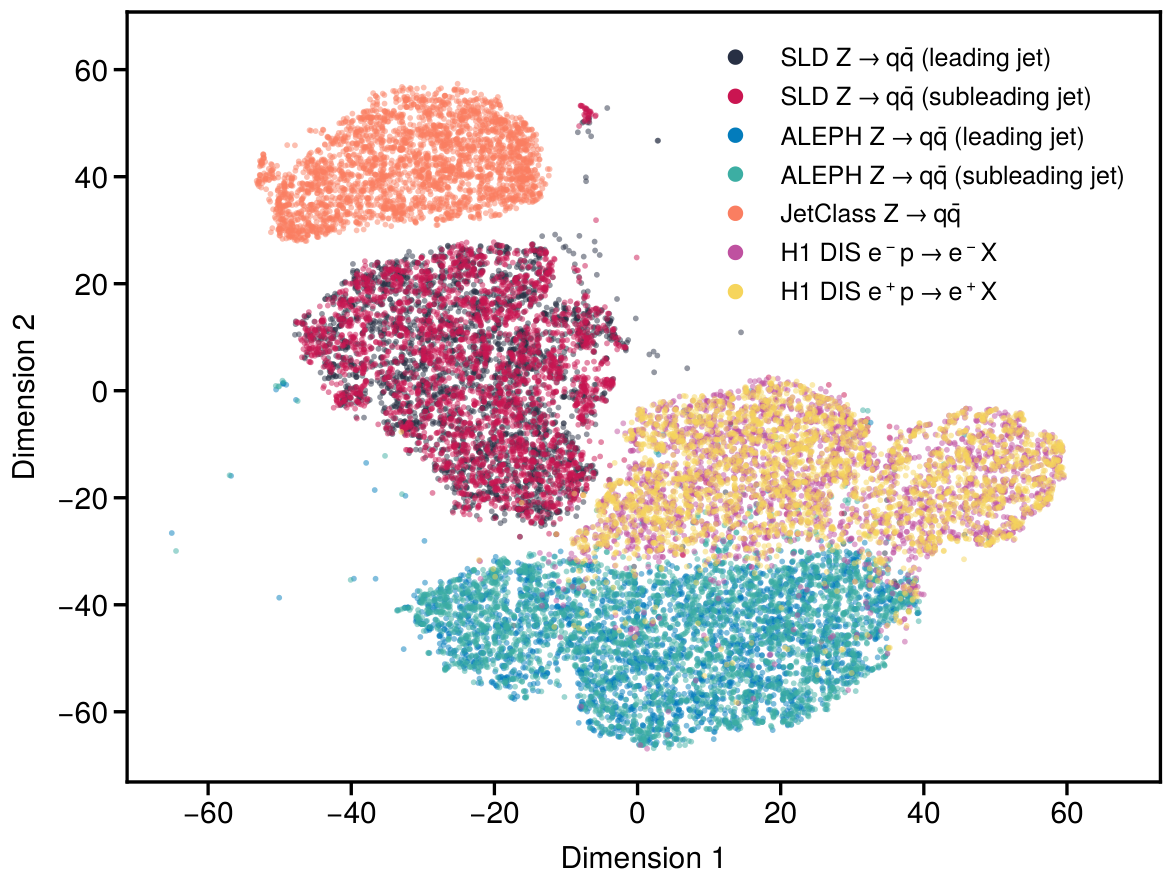
\includegraphics[width=\linewidth,height=48mm,keepaspectratio]{figures/embedding_tsne_m.png}

      {\tiny\textit{Fig.~6, arXiv:2606.00224: t-SNE visualization of OmniLearned jet embeddings.}\par}
    \end{column}

    \begin{column}{0.30\textwidth}
      {\small\textbf{t-SNE of jet embeddings}}\par
      \begin{itemize}
        \setlength{\itemsep}{0.8mm}
        \item Learned jet embeddings are projected to 2D for visualization.
        \item Jets with similar learned features appear nearby.
        \item Similar physics topologies group together in embedding space.
      \end{itemize}
    \end{column}
  \end{columns}
  \vfill

  \slideheaderfooter
\end{frame}
